\documentclass[12pt,a4]{article}
\usepackage{physics, amsmath,amsfonts,amsthm,amssymb, mathtools,steinmetz, gensymb, siunitx}	% LOADS USEFUL MATH STUFF
\usepackage{xcolor,graphicx}
\usepackage[left=45pt, top=20pt, right=45pt, bottom=45pt ,a4paper]{geometry} 				% ADJUSTS PAGE
\usepackage{setspace}
\usepackage{caption}
\usepackage{tikz}
\usepackage{pgf,tikz,pgfplots,wrapfig}
\usepackage{mathrsfs}
\usepackage{fancyhdr}
\usepackage{float}
\usepackage{array}
\usepackage{booktabs,multirow}
\usepackage{bm}

\usetikzlibrary{decorations.text, calc}
\pgfplotsset{compat=1.7}

\usetikzlibrary{decorations.pathreplacing,decorations.markings}
\usepgfplotslibrary{fillbetween}

\newcommand{\vect}[1]{\boldsymbol{#1}}

\usepackage{hyperref}
%\usepackage[style= ACM-Reference-Format, maxbibnames=6, minnames=1,maxnames = 1]{biblatex}
%\addbibresource{references.bib}


\AtBeginDocument{\hypersetup{pdfborder={0 0 0}}}

\title{
\textsc{Topic 3}
}
\author{\textsc{J L Gouws}
}
\date{\today
\\[1cm]}



\usepackage{graphicx}
\usepackage{array}




\begin{document}
\thispagestyle{empty}

\maketitle

\begin{enumerate}
  \item
    \begin{enumerate}
      \item
        Figure~\ref{fig:1a} shows the errors made when evolving a logistic eqution with an Euler evolver for different time steps.
        \begin{figure}[H]
          \centering
          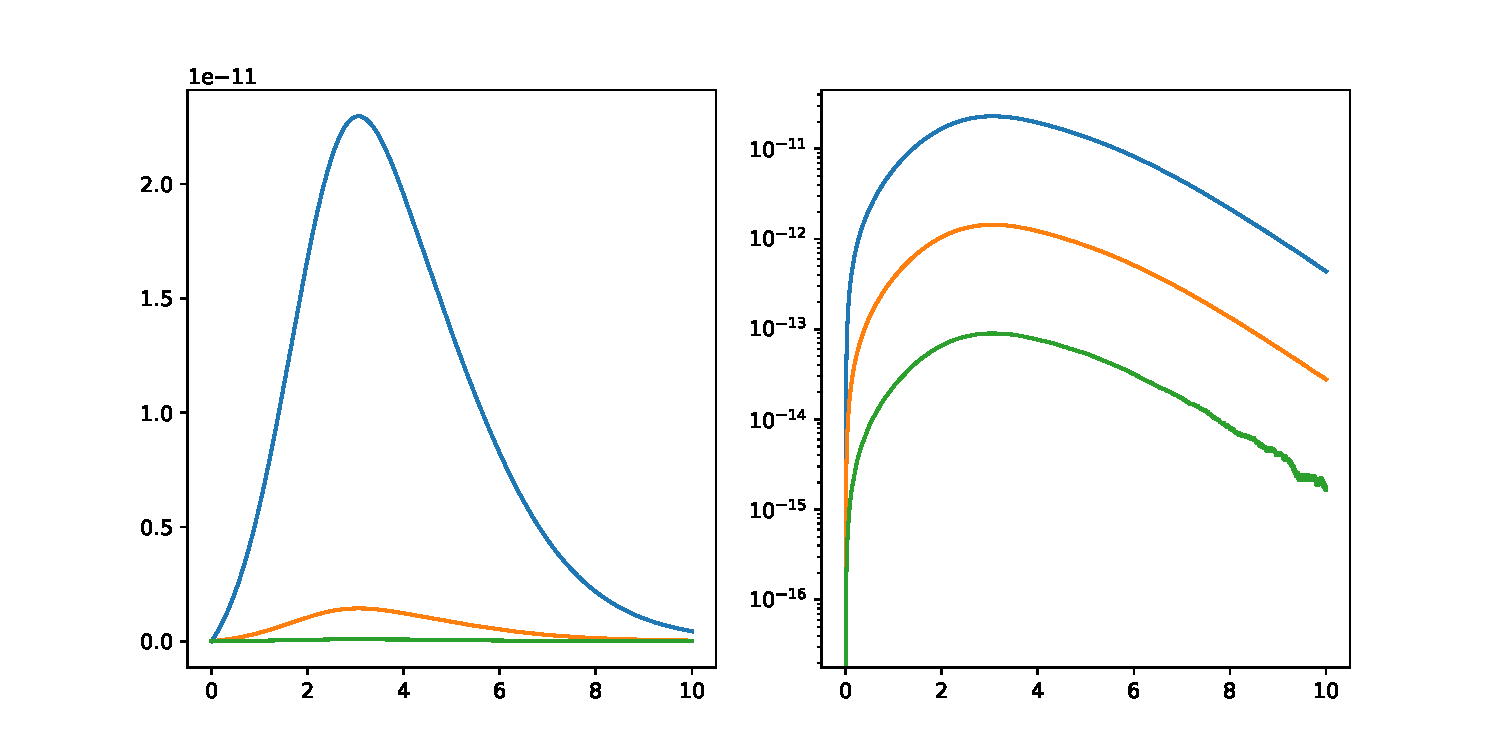
\includegraphics[scale = 0.7]{../figs/1a.pdf} 
          \caption{Global errors for Euler evolution using of a logistic equation different time steps}
          \label{fig:1a}
        \end{figure}

      \item
        Figure~\ref{fig:1b} shows the relationship between the errors when evolving with different time steps.
        Halving the time step decreases the error by a factor of two.
        This relationship confirms that the Euler method is first order--halving the time-step halves the error.

        \begin{figure}[H]
          \centering
          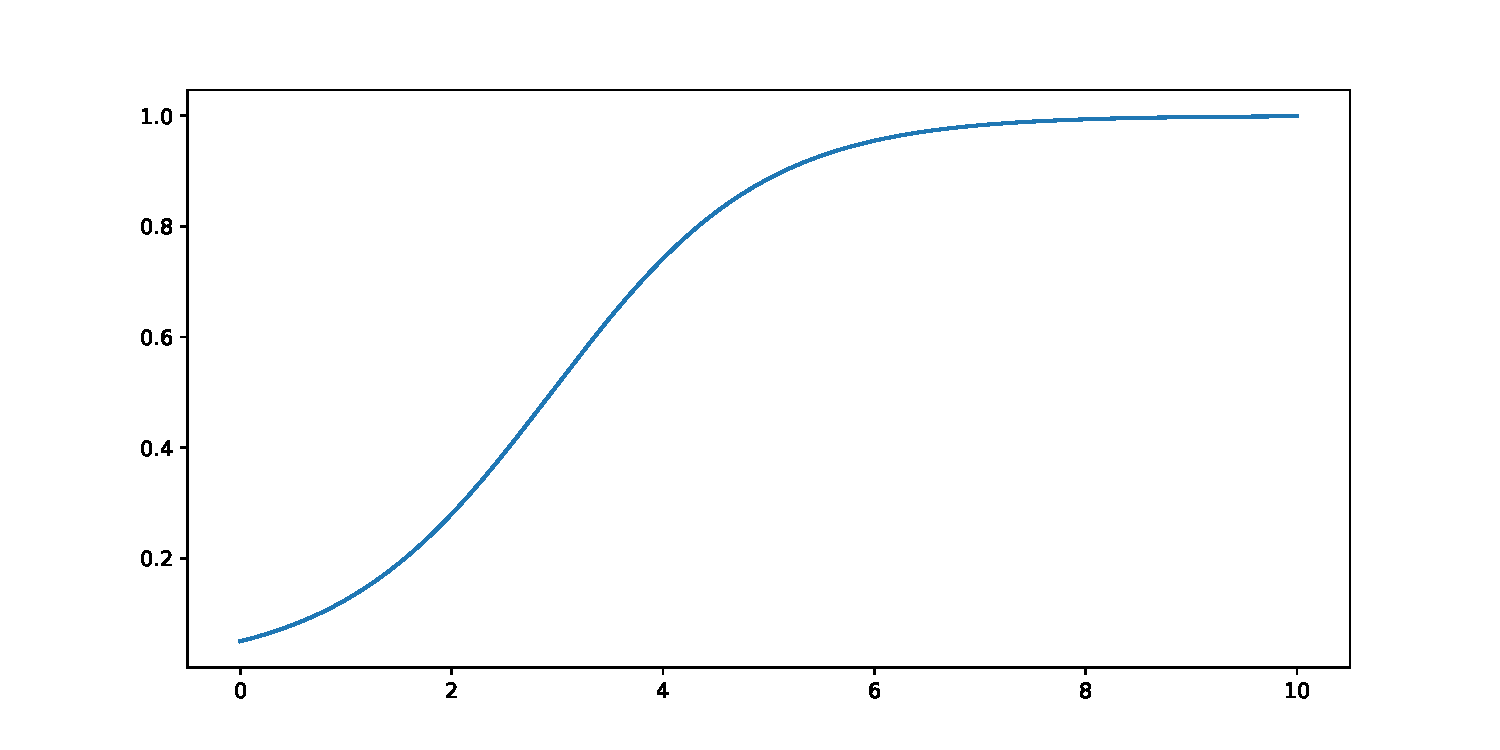
\includegraphics[scale = 0.7]{../figs/1b.pdf}
          \caption{Scaled global errors for Euler evolution of a logistic equation using different time steps}
          \label{fig:1b}
        \end{figure}

      \item
        Figure~\ref{fig:1c} compares the actual global error of the logistic problem's Euler evolution against the error estimated with the Richardson extrapolation.
        \begin{figure}[H]
          \centering
          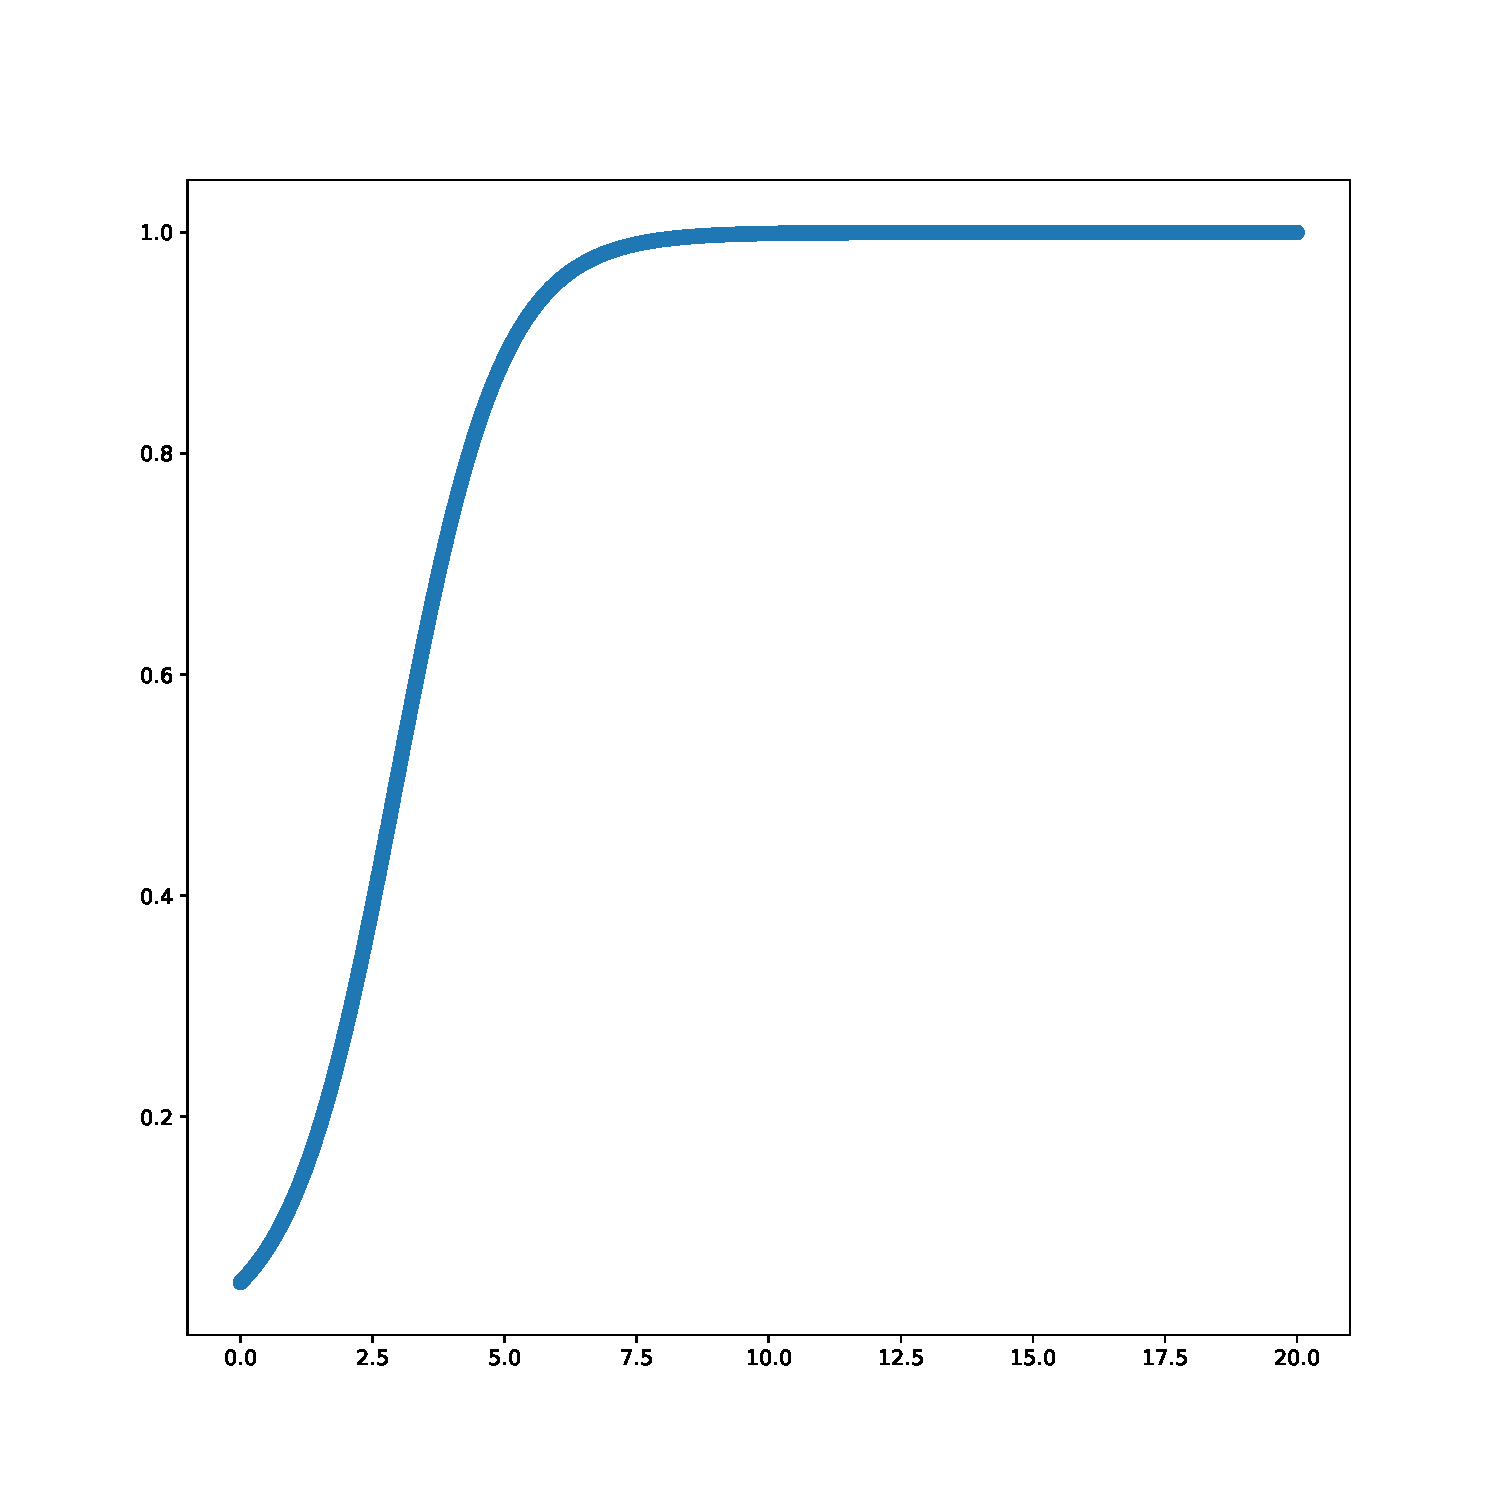
\includegraphics[scale = 0.6]{../figs/1c.pdf}
          \caption{Comparison of the actual error with the difference between the Richardson extrapolation and numerical solution}
          \label{fig:1c}
        \end{figure}


    \end{enumerate}
  \item
    \begin{enumerate}
      \item
        Figure~\ref{fig:2a} shows the errors made when evolving a logistic equation with an RK2 evolver for different time steps.
        \begin{figure}[H]
          \centering
          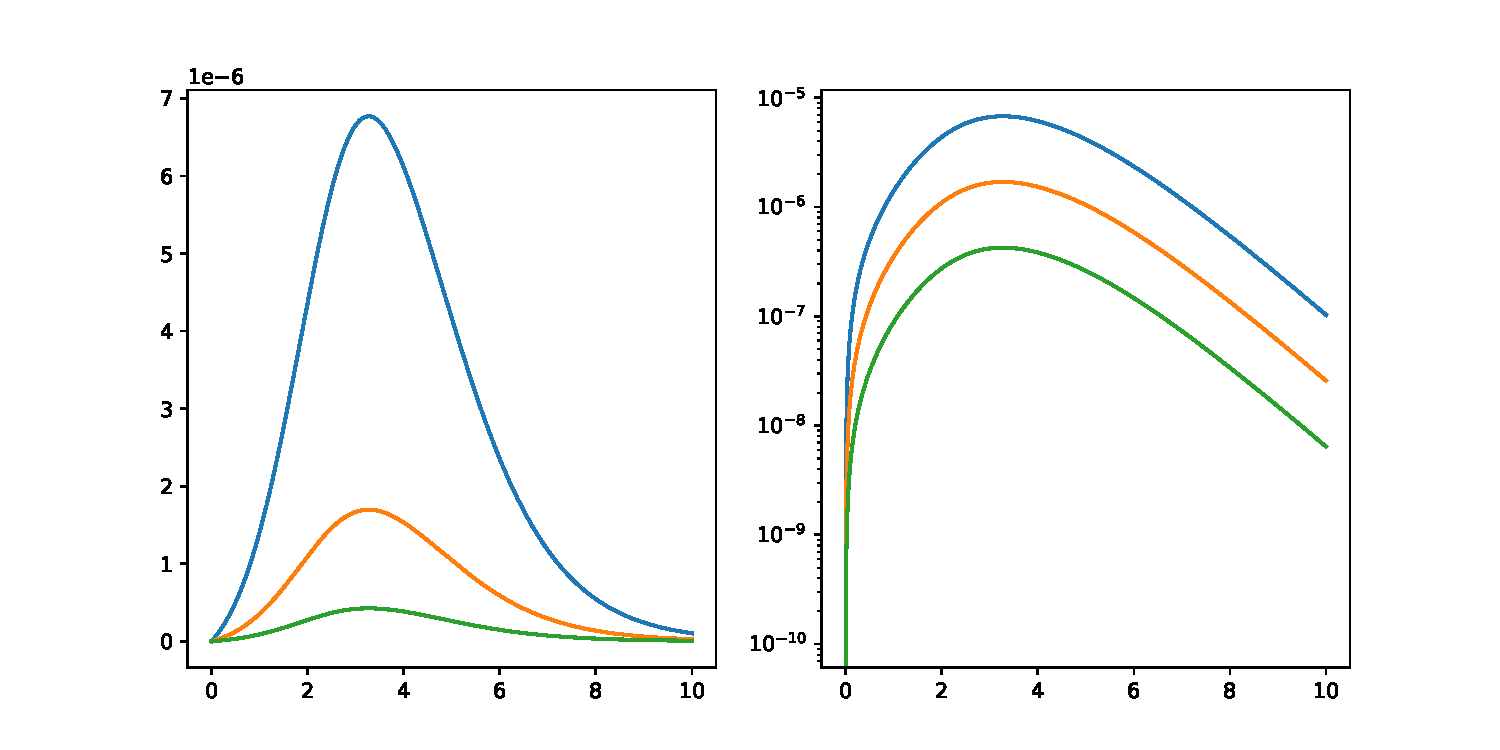
\includegraphics[scale = 0.7]{../figs/2a.pdf}
          \caption{Global errors for RK2 evolution using of a logistic equation different time steps}
          \label{fig:2a}
        \end{figure}

      \item
        Figure~\ref{fig:2b} shows the relationship between the errors when evolving with different time steps.
        Halving the time step decreases the error by a factor of four.
        This relationship confirms that the second order Runge-Kutta method is indeed second order.
        Halving the time-step decreases the error by $2^p = 4$.
        \begin{figure}[H]
          \centering
          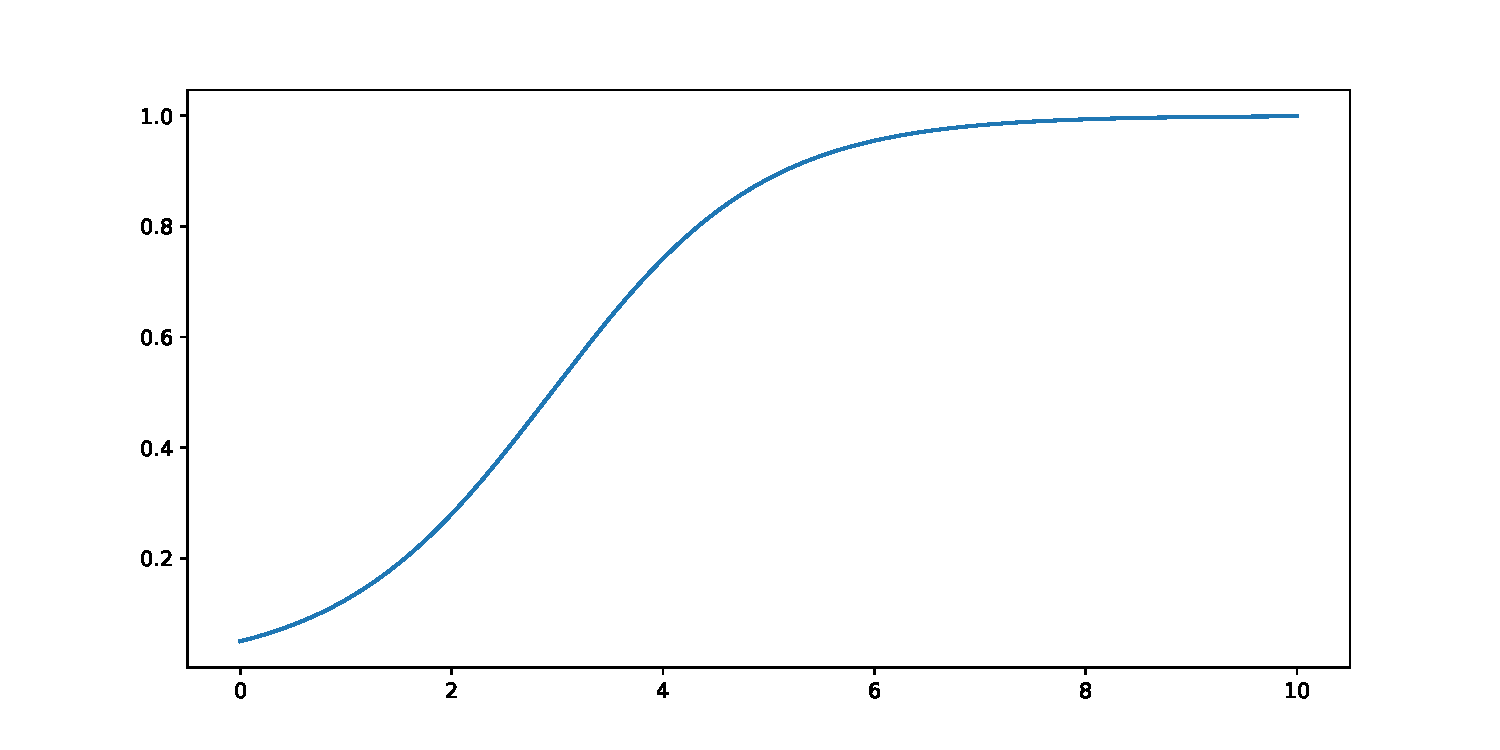
\includegraphics[scale = 0.7]{../figs/2b.pdf}
          \caption{Scaled global errors for RK2 evolution of a logistic equation using different time steps}
          \label{fig:2b}
        \end{figure}
      \item
        Figure~\ref{fig:2c} compares the actual global error of the logistic problem's RK2 evolution against the error estimated with the Richardson extrapolation.
        \begin{figure}[H]
          \centering
          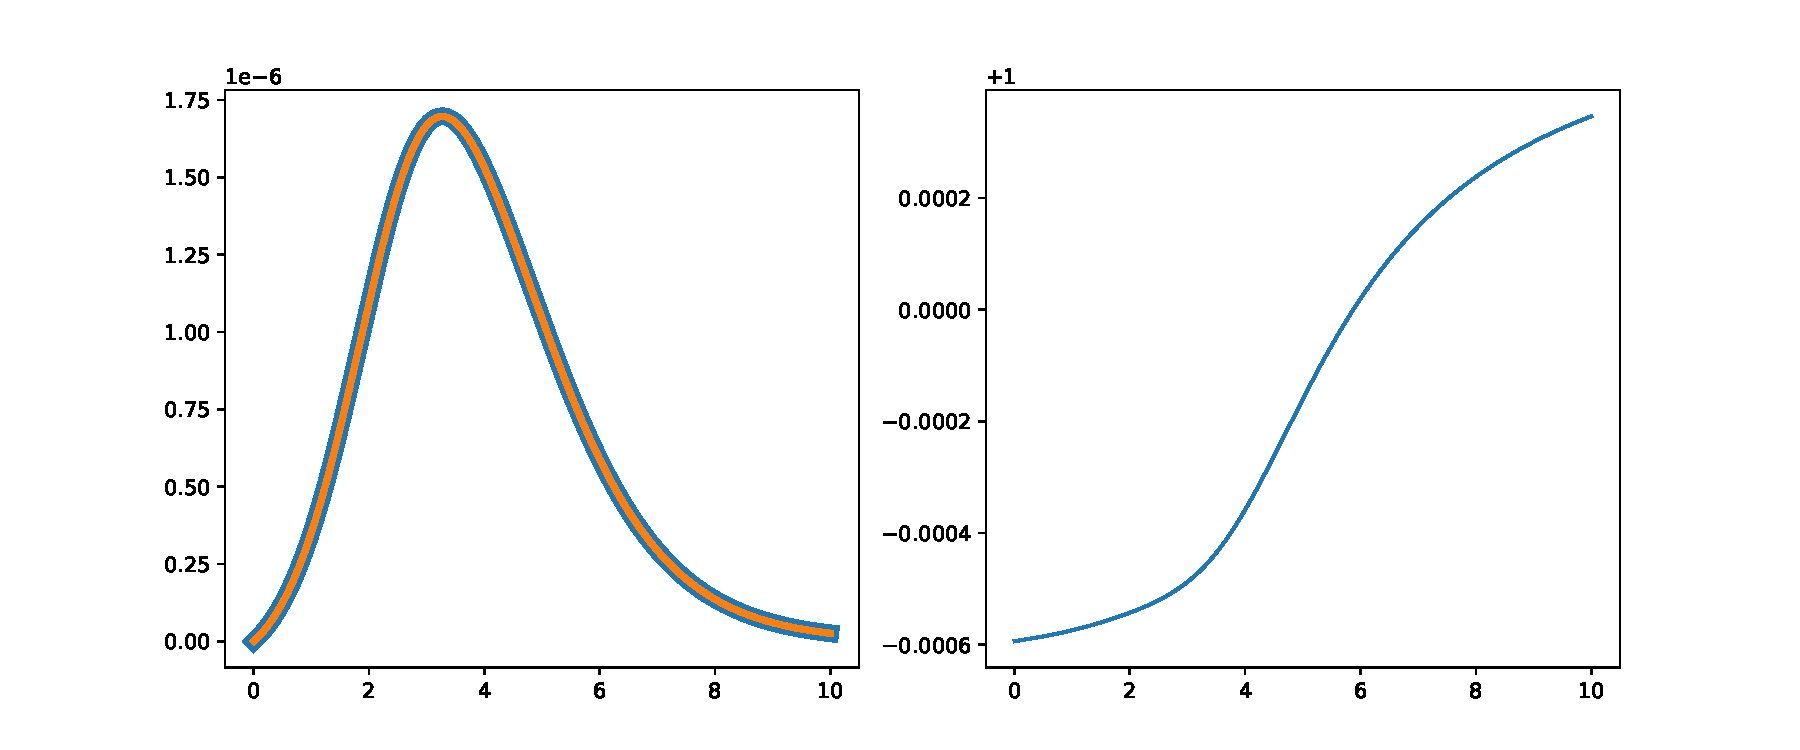
\includegraphics[scale = 0.6]{../figs/2c.pdf}
          \caption{Comparison of the actual error with the difference between the Richardson extrapolation and numerical the solution}
          \label{fig:2c}
        \end{figure}
  \end{enumerate}
  \item
    Figure~\ref{fig:3} shows that the maximum error occurs near the point in the solution with the largest derivative.
    \begin{figure}[H]
      \centering
      \includegraphics[scale = 0.7]{../figs/3.pdf}
      \caption{Comparison of the actual error and the Richardson extrapolation's derivative}
      \label{fig:3}
    \end{figure}
  \item
    Figure~\ref{fig:4} gives a log-log plot of the evolution time step agains the error's L2-norm.
    The line for the Euler method has a gradient close to one; The line for the RK2 method has gradient close to two.
    \begin{figure}[H]
      \centering
      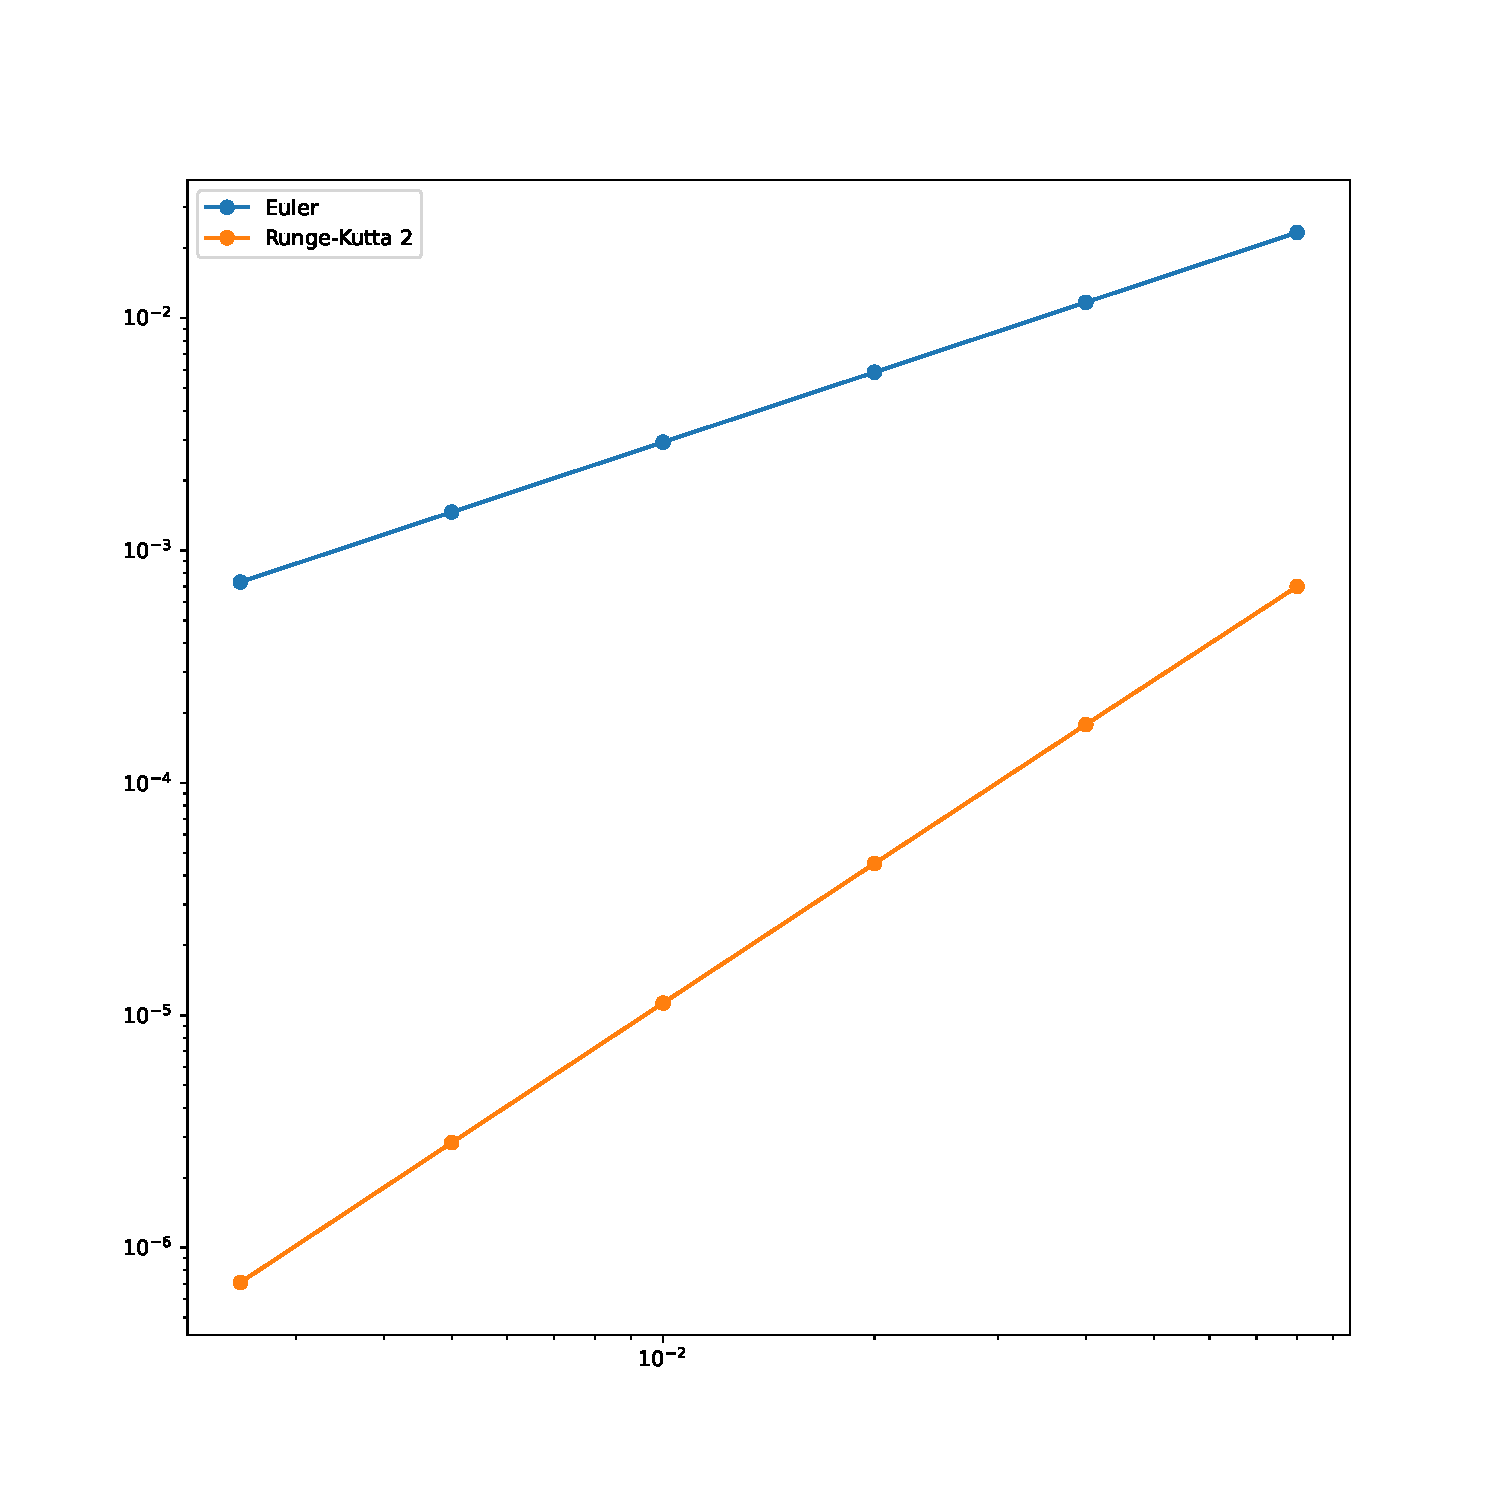
\includegraphics[scale = 0.7]{../figs/4.pdf}
      \caption{Error's L2-norm as a function of the numerical approximation's time step}
      \label{fig:4}
    \end{figure}
\end{enumerate}

\end{document}
